\documentclass[svgnames,14pt]{beamer}
\usepackage{caption}
\usepackage{graphicx}
\usepackage{xcolor}
\usepackage{wrapfig}
\usepackage{algorithm}
\usepackage{algpseudocode}
\title{Genomes Comparision via de Bruijn graphs}
\author{Student: Ilya Minkin \\ Advisor: Son Pham}
\institute{St. Petersburg Academic University}
\date{June 4, 2012}
\algnotext{EndFor}
\algnotext{EndIf}
\algnotext{EndWhile}
\setbeamertemplate{footline}[frame number]
\setbeamertemplate{navigation symbols}{}
\setbeamertemplate{caption}[numbered]
\begin{document}
\def\braces#1{[#1]}
\newenvironment{changemargin}[2]{% 
  \begin{list}{}{% 
    \setlength{\topsep}{0pt}% 
    \setlength{\leftmargin}{#1}% 
    \setlength{\rightmargin}{#2}% 
    \setlength{\listparindent}{\parindent}% 
    \setlength{\itemindent}{\parindent}% 
    \setlength{\parsep}{\parskip}% 
  }% 
  \item[]}{\end{list}}
\maketitle

\begin{frame}
\frametitle{Synteny Blocks: Algorithmic challenge}
\begin{itemize}
\item Suppose that we are given two genomes
\item The question is: how are they evolutionary related to each other?
\item In order to do rearrangements analysis we must decompose genomes into synteny blocks
\item Synteny blocks are evolutionary conserved segments of the genome
\item These blocks cover most of the genome
\item Occur in both genomes with possible variations
\end{itemize}
\end{frame}

\begin{frame}
\frametitle{Academic Project}
Project: Identify synteny blocks for duplicated genomes represented as sequences of \textbf{nucleotides}.
\begin{itemize}
\item \textbf{None} of the previous synteny blocks reconstruction software (DRIMM-Synteny (Pham And Pevzner 2010) included) can 
efficiently solve this problem. 
\item DRIMM-Synteny can find the synteny blocks for complicated genomes. But:
\pause \item It requires the genome to be represented as sequence of genes. 
\end{itemize}
\end{frame}

\begin{frame}
\frametitle{General Idea: de Bruijn Graph}
\begin{itemize}
\item We are given an alphabet \( \Sigma \) and a string \( S \) over it, \(|\Sigma| = m \)
\item A substring \( T, \, |T| = k \) is called \textit{k-mer}
\item De Bruijn graph is a multigraph \( G_{k} = (V, E) \), where \\
\( V = \Sigma^{k - 1} = \) \{all possible \( (k - 1) \)-mers\} \\
\item If \(k\)-mer \( T \) is presented in \( S \), then we add an oriented edge \( (T[1, k - 1], T[2, k]) \) to the graph
\item Create de Bruijn graph from the nucleotide sequence
\item Conserved regions will yield non-branching paths
\end{itemize}
\end{frame}

\begin{frame}
\frametitle{Challenges}
\begin{itemize}
\item Variations in synteny blocks generate cycles, so we need to simplify the graph
\item Double strandness: conserved regions may occur on both strands. Example: \\
5' \textcolor{Green}{AACC}GGTT 3' \\
3' TTGG\textcolor{Green}{CCAA} 5' \\
Such blocks are reverse complementary to each other \( \Rightarrow \) no non-branching paths
\item Spurious similarity
\item Memory efficiency
\end{itemize}
\end{frame}

\begin{frame}
\frametitle{Colored graph}
\begin{itemize}
\item We use colored de Bruijn graphs \\
\braces{Iqball et al., 2012} to handle double-strandness
\item Suppose that \( S^{+} \) and \( S^{-} \) are positive and negative strands of the chromosome
\item Colored de Bruijn graph  is a multigraph \( G_{k} = (V, E) \) where \( V =  \Sigma^{k - 1} \)
\item For each \(k\)-mer \(T^{+}\) in \(S^{+}\) add edge \( (T^{+}[1, k - 1], T^{+}[2, k]) \) to \( G_{k} \) and mark it \\ \textit{blue}
\item For each \(k\)-mer \(T^{-}\) in \(S^{-}\) add edge \( (T^{-}[1, k - 1], T^{-}[2, k]) \) to \( G_{k} \) and mark it \\ \textit{red}
\end{itemize}
\end{frame}

\begin{frame}
\frametitle{Edge labeling}
\begin{itemize}
\item Note that our graph is built from a string, not set of reads
\item Each walk in the graph represents a string
\item We are interested only in walks that represent substrings of the source string
\item Assign to each edge \( e \) label \( L(e) = \) position of the corresponding  \(k\)-mer on the positive strand
\item Walk  \( W = ( v_{1} \, e_{1} \, v_{2} \, e_{2} \, ... ) \) is considered valid iff: \\
1. \( e_{i} \) and \( e_{i + 1} \) are of the same color \\
2. \( | L(e_{i}) - L(e_{i + 1}) | = 1 \)
\end{itemize}
\end{frame}

\begin{frame}
\frametitle{Example}
\begin{changemargin}{-1.cm}{-1.cm}
\begin{figure}
\centering
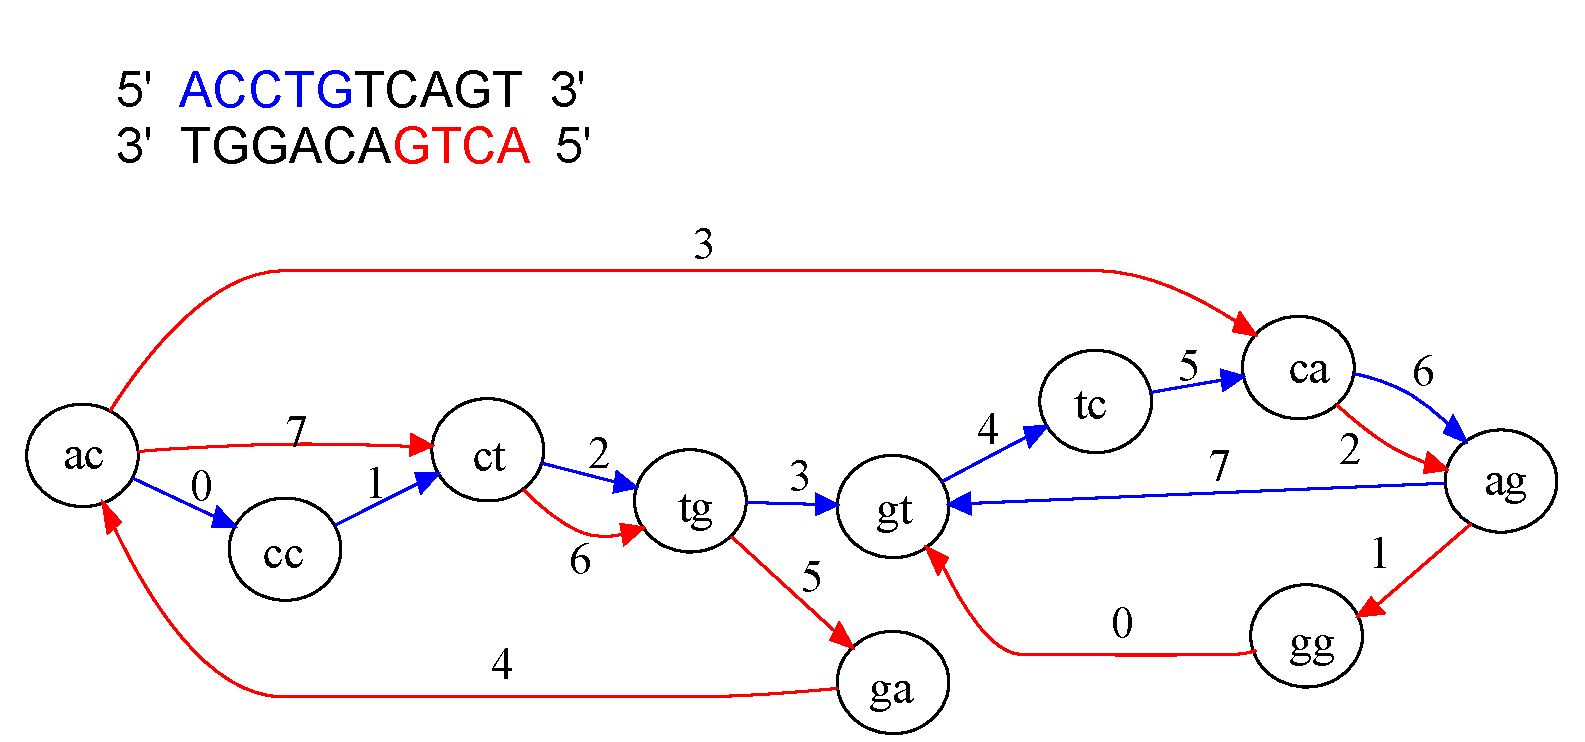
\includegraphics[scale = 0.480]{Figure1.pdf}
\small \caption{Colored de Bruijn graph built from two strands}
\end{figure}
\end{changemargin}
\end{frame}

\begin{frame}
\frametitle{Graph simplification}
\begin{itemize}
\item Bulges spoil long non-branching paths and indicate indels/mismatches
\item A pair of walks \((W_{1}, W_{2})\) is a bulge iff: \\
1) Start and end vertices of  \(W_{1} \) and  \(W_{2}\) coincide\\
2) \(W_{1} \) and  \(W_{2}\) have exactly 2 common vertices \\
3) There are no edges \(u \in W_{1} \) and \( v \in W_{2}\) such that \(L(u) = L(v) \) \\
4) \(|W_{1}|  \leq \delta \) and \(|W_{2}| \leq \delta \)
\end{itemize}
\begin{changemargin}{-1.cm}{-1.cm}
\begin{figure}
\centering
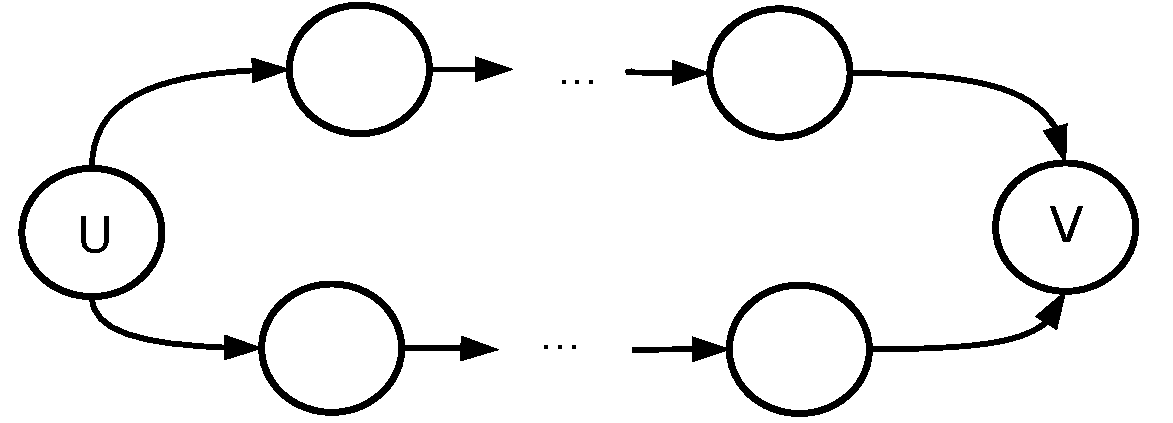
\includegraphics[scale = 0.30]{Figure2.pdf}
\small \caption{A bulge}
\end{figure}
\end{changemargin}
\end{frame}

\begin{frame}
\frametitle{General pipeline}
\begin{itemize}
\item Build de Bruijn graph from the genome
\item Remove bulges (BFS-like algorithm)
\item Bulges are removed by replacing long branches with shorter ones
\item Output non-branching paths
\end{itemize}
\begin{changemargin}{-1.cm}{-1.cm}
\begin{figure}
\centering
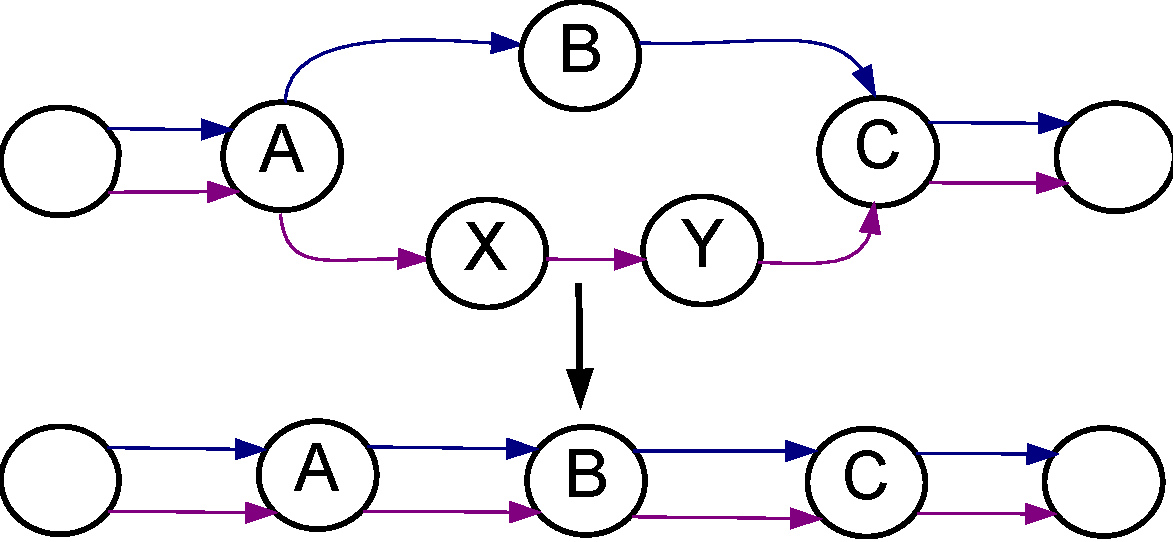
\includegraphics[scale = 0.45]{Figure3.pdf}
\small \caption{Bulge removal illustration}
\end{figure}
\end{changemargin}
\end{frame}

\begin{frame}
\frametitle{Parameters selection}
\begin{itemize}
\item How should we choose \(K\) and \(\delta\)?
\item Duplicated genes can have no long (\(K > 50 \)) shared \(K\) - mers
\item Big \(K \sim 50\) -- we find only few synteny blocks
\item Small \(K \sim 10\) and small \(\delta \sim 15\) -- we find very short synteny blocks
\item Small \(K \sim 10\) and big \(\delta \sim 200 \) -- the genome will be disrupted completely
\pause \item Solution -- do simplification in multiple stages 
\end{itemize}
\end{frame}

\begin{frame}
\frametitle{New pipeline}
\begin{itemize}
\item General idea -- "align" similar regions first, then glue them together into synteny blocks
\item Start with small \(K\) and small \(\delta\) to smooth duplicated regions and obtain long \(K\)-mers
\item Rebuild and simplify the graph with higher \(K\) and \(\delta\)
\item Continue this process several times
\item Final step can be done with \(K \sim \) several hundreds
\end{itemize}
\end{frame}

\begin{frame}
\frametitle{Experiment}
\begin{itemize}
\item We have attempted to identify duplications in \emph{Arabidopsis thaliana}
\item Arabidopsis is known to be highly duplicated genome \braces{Arabidopsis Genome Initiative}
\item Size of the genome is \( \sim 120 \, Mbp \)
\item We used 4 stages and following parameters:
\end{itemize}
\begin{center}
\begin{tabular}{|c|c|c|}
\hline
Stage number & \(K\) & \(\delta\) \\
\hline
1 & 15 & 150 \\
\hline
2 & 50 & 500\\
\hline
3 & 100 & 1000\\
\hline
4 & 500 & 5000\\
\hline
\end{tabular}
\end{center}
\end{frame}

\begin{frame}
\frametitle{Computation results}
\begin{itemize}
\item We have found \(4722\) synteny blocks in Arabidopsis
\item These blocks cover \(28 \, \%\) of the genome
\item Minimum length of the block is \(1000 \, bp\)
\item Largest block found has length \(\sim 95 \, 000 \, bp\)
\item We tried to verify blocks by aligning instances of the same block
\item At least \(87 \, \%\) of blocks have \(50 \, \%\) of exact matches
\end{itemize}
\end{frame}

\begin{frame}
\frametitle{Computation results}
\begin{figure}
\centering
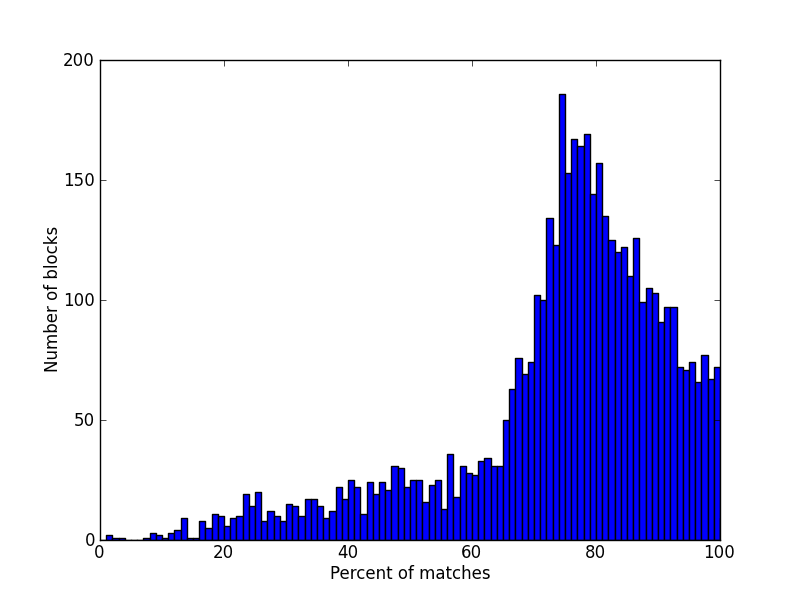
\includegraphics[scale = 0.480]{blocks_alignments.png}
\small \caption{Matches percent vs. number of blocks plot}
\end{figure}
\end{frame}

\begin{frame}
\frametitle{Computation results}
\begin{figure}
\centering
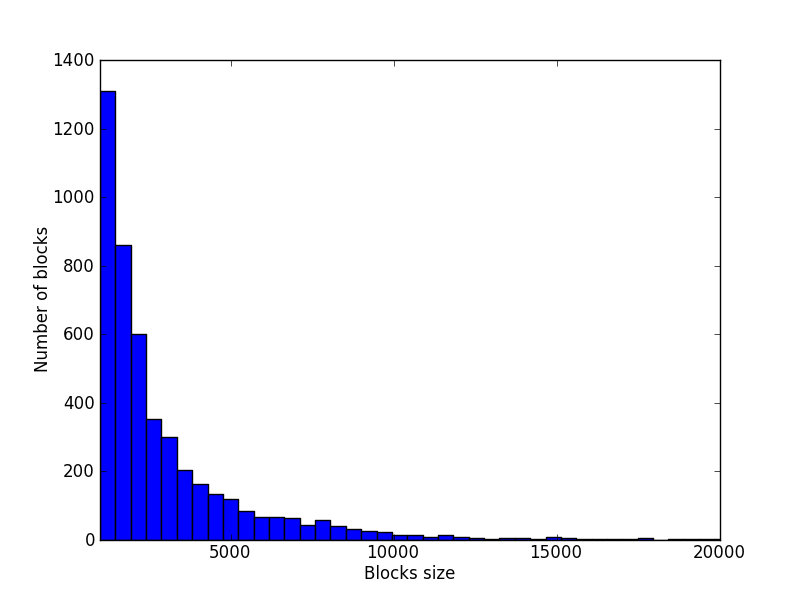
\includegraphics[scale = 0.480]{blocks_len_distrib.png}
\small \caption{Synteny blocks length distribution}
\end{figure}
\end{frame}

\begin{frame}
\frametitle{Summary}
\begin{itemize}
\item We have covered 28 \% of Arabidopsis genome with synteny blocks
\item But we have missed some duplicated regions, described in \braces{Arabidopsis Genome Initiative}
\item Most of the blocks are short (\(< 5000 \,  bp\))
\item We must improve coverage and "lengthen" the blocks
\end{itemize}
\pause
Near plans:
\begin{itemize}
\item Improve performance
\item Examine other genomes
\item Optimize algorithms to handle larger genomes
\end{itemize}
\end{frame}

\begin{frame}
\frametitle{Applications}
\begin{itemize}
\item A multiple sequence alignment program
\item Finding the synteny blocks for complicated genomes (Mammalian),
possible collaboration -- Jian Ma.
\item Tool for genomes vs genomes and/or assemblies vs.
assemblies and/or assemblies vs. genomes comparisions.
\end{itemize}
\end{frame}

\begin{frame}
\frametitle{References}
\begin{itemize}
\item 1. Pevzner P and Tesler G, (2003) Human and mouse genomic sequences reveal extensive breakpoint reuse in mammalian evolution. 
\item 2. Pham S and Pevzner P, (2010) DRIMM-Synteny: Decomposing Genomes into Evolutionary Conserved Segments
\item 3. Iqbal Z, Caccamo M, Turner I, Flicek P, McVean G, (2012) De novo assembly and genotyping of variants using colored de Bruijn graphs
\item 4. Arabidopsis Genome Initiative, (2000) Analysis of the genome sequence of the flowering plant Arabidopsis thaliana
\end{itemize}
\end{frame}

\begin{center}
\hfill \huge \\
\vspace{60pt}
Thank you!
\end{center}

\end{document}
